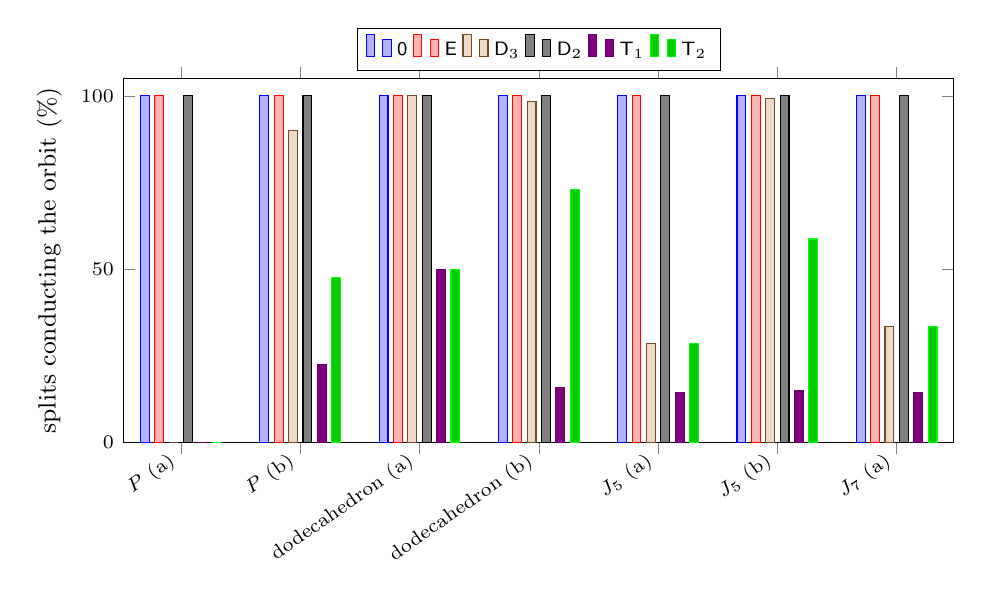
\begin{tikzpicture}
\begin{axis}[ybar,width=\textwidth,height=6.2cm,bar width=3.2pt,ymin=0,ymax=105,ylabel={splits conducting the orbit (\%)},symbolic x coords={Pa,Pb,Dodecaa,Dodecab,J5a,J5b,J7a},xtick=data,xticklabels={$P$ (a),$P$ (b),dodecahedron (a),dodecahedron (b),$J_5$ (a),$J_5$ (b),$J_7$ (a)},x tick label style={font=\scriptsize,rotate=35,anchor=east},tick label style={font=\scriptsize},label style={font=\small},legend style={font=\scriptsize,at={(0.5,1.02)},anchor=south,legend columns=6},enlarge x limits=0.08]
\addplot coordinates {(Pa,100.0) (Pb,100.0) (Dodecaa,100.0) (Dodecab,100.0) (J5a,100.0) (J5b,100.0) (J7a,100.0)};
\addplot coordinates {(Pa,100.0) (Pb,100.0) (Dodecaa,100.0) (Dodecab,100.0) (J5a,100.0) (J5b,100.0) (J7a,100.0)};
\addplot coordinates {(Pa,0.0) (Pb,90.0) (Dodecaa,100.0) (Dodecab,98.3) (J5a,28.6) (J5b,99.2) (J7a,33.3)};
\addplot coordinates {(Pa,100.0) (Pb,100.0) (Dodecaa,100.0) (Dodecab,100.0) (J5a,100.0) (J5b,100.0) (J7a,100.0)};
\addplot coordinates {(Pa,0.0) (Pb,22.5) (Dodecaa,50.0) (Dodecab,15.7) (J5a,14.3) (J5b,14.8) (J7a,14.3)};
\addplot coordinates {(Pa,0.0) (Pb,47.5) (Dodecaa,50.0) (Dodecab,73.0) (J5a,28.6) (J5b,58.7) (J7a,33.3)};
\legend{$\mathsf{0}$,$\mathsf{E}$,$\mathsf{D}_3$,$\mathsf{D}_2$,$\mathsf{T}_1$,$\mathsf{T}_2$}
\end{axis}
\end{tikzpicture}
